% XeLaTeX: ./build.ps1 or bash build.sh.
\documentclass[12pt,a4paper]{article}
\usepackage{fontspec,polyglossia}
\setdefaultlanguage{russian}
\setotherlanguage{english}
\setmainfont{Times New Roman}
\usepackage{amsmath,amssymb,graphicx,booktabs,float,geometry,setspace}
\usepackage[unicode,hidelinks]{hyperref}
\geometry{left=25mm,right=20mm,top=20mm,bottom=20mm}
\onehalfspacing
\setlength{\parindent}{1.25cm}
\setlength{\emergencystretch}{2em}
\graphicspath{{figures/}}
% Generated by lab4.py.
\newcommand{\FringeWidth}{5{,}500}
\newcommand{\SourceAngle}{0{,}157564}
\newcommand{\SingleZero}{22{,}000}
\newcommand{\SingleWidth}{44{,}000}
\newcommand{\AiryRadius}{6{,}708}
\newcommand{\GratingAngle}{3{,}152859}
\newcommand{\VisibilityError}{0{,}00002}
\newcommand{\SpacingError}{0{,}0050}


\begin{document}
\begin{titlepage}
\begin{center}
\begin{spacing}{1.3}
\textbf{МИНИСТЕРСТВО ОБРАЗОВАНИЯ РЕСПУБЛИКИ БЕЛАРУСЬ}\\[0.25cm]
\textbf{БЕЛОРУССКИЙ ГОСУДАРСТВЕННЫЙ УНИВЕРСИТЕТ}\\[0.25cm]
\textbf{ФАКУЛЬТЕТ МЕХАНИКО-МАТЕМАТИЧЕСКИЙ}\\[0.25cm]
\textbf{Кафедра веб-технологий и компьютерного моделирования}
\end{spacing}
\vspace{4.2cm}
\textbf{ВОЛНОВЫЕ СВОЙСТВА СВЕТА}\\[0.2cm]
\textbf{ИНТЕРФЕРЕНЦИЯ, ПОЛЯРИЗАЦИЯ И ДИФРАКЦИЯ}\\[0.4cm]
Лабораторная работа № 4
\end{center}
\vspace{3.4cm}
\noindent\hspace*{0.48\textwidth}\begin{minipage}{0.52\textwidth}
\begin{spacing}{1.0}
Панасика Владислава Александровича\\
обучающегося 4 курса специальности\\
«Математика и компьютерные науки»\\[0.6cm]
Научный руководитель:\\
ассистент КФОиПИ,\\
Полякова Яна Владимировна
\end{spacing}
\end{minipage}
\vfill
\begin{center}Минск, 2026\end{center}
\end{titlepage}
\setcounter{page}{2}
\tableofcontents
\clearpage

\section{Интерференция: контраст и ширина полос}
Исследуется распределение интенсивности при $\lambda=550$ нм,
$I_0=1$ в относительных единицах. Выбраны расстояние до экрана
$L=2$ м и расстояние между источниками $d=0{,}20$ мм.
В параксиальной модели $\Delta=dx/L$:
\begin{equation}
 I(x)=I_1+I_2+2\sqrt{I_1I_2}\cos\frac{2\pi dx}{\lambda L},\qquad
 V=\frac{I_{\max}-I_{\min}}{I_{\max}+I_{\min}}
 =\frac{2\sqrt{I_1I_2}}{I_1+I_2}.
\end{equation}
\begin{figure}[H]
\centering
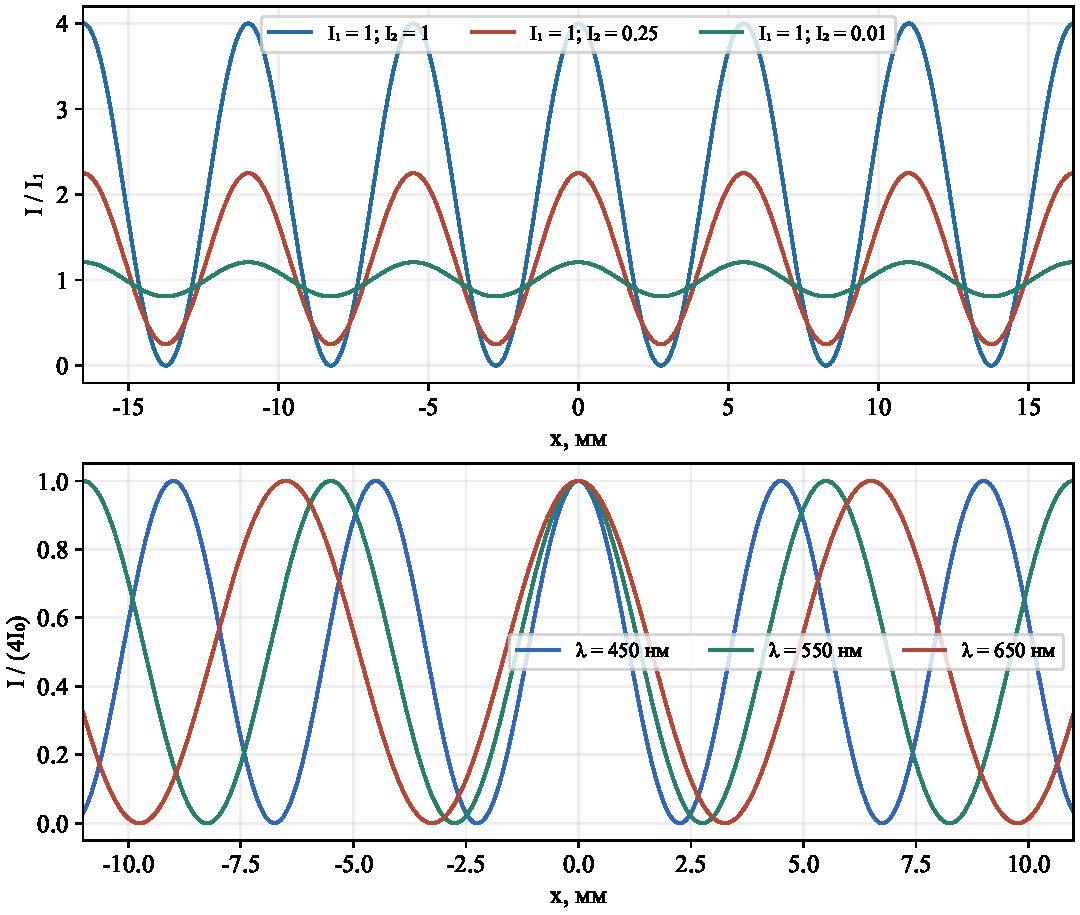
\includegraphics[width=0.75\textwidth]{task1_visibility.pdf}
\caption{Влияние соотношения интенсивностей и длины волны на полосы.}
\end{figure}
\begin{table}[H]
\centering
\caption{Результаты при $I_1=1$; $\Delta x$ найдено по максимумам графика}
\begin{tabular}{rrrrrr}
\toprule
$I_2$ & $I_{\max}$ & $I_{\min}$ & $V_{\mathrm{теор}}$ & $V_{\mathrm{сетка}}$ & $\Delta x$, мм\\
\midrule
\input results/visibility_rows.tex
\bottomrule
\end{tabular}
\end{table}
Ширина полосы $\Delta x=\lambda L/d=\FringeWidth$ мм одинакова
для трёх соотношений интенсивностей. Относительная ошибка определения
$V$ по сетке не превышает \VisibilityError\,\%, ширины --- \SpacingError\,\%.
Это ошибки дискретизации, а не погрешности измерений.

Наилучший контраст $V=1$ получается при равных интенсивностях,
когерентности и параллельной поляризации волн. При $I_1\gg I_2$
полосы слабо выражены. Для 450, 550 и 650 нм ширина равна соответственно
4,5; 5,5 и 6,5 мм: более длинная волна даёт более широкие полосы.
Эффект используется для измерения длины волны и малых перемещений.

\clearpage
\section{Два когерентных точечных источника}
Для равных интенсивностей $I_1=I_2=I_0=1$ угловое распределение:
\begin{equation}
 I(\theta)=4I_0\cos^2\frac{\pi d\sin\theta}{\lambda},\qquad
 d\sin\theta_m=m\lambda,\quad m\in\mathbb Z.
\end{equation}
\begin{figure}[H]
\centering
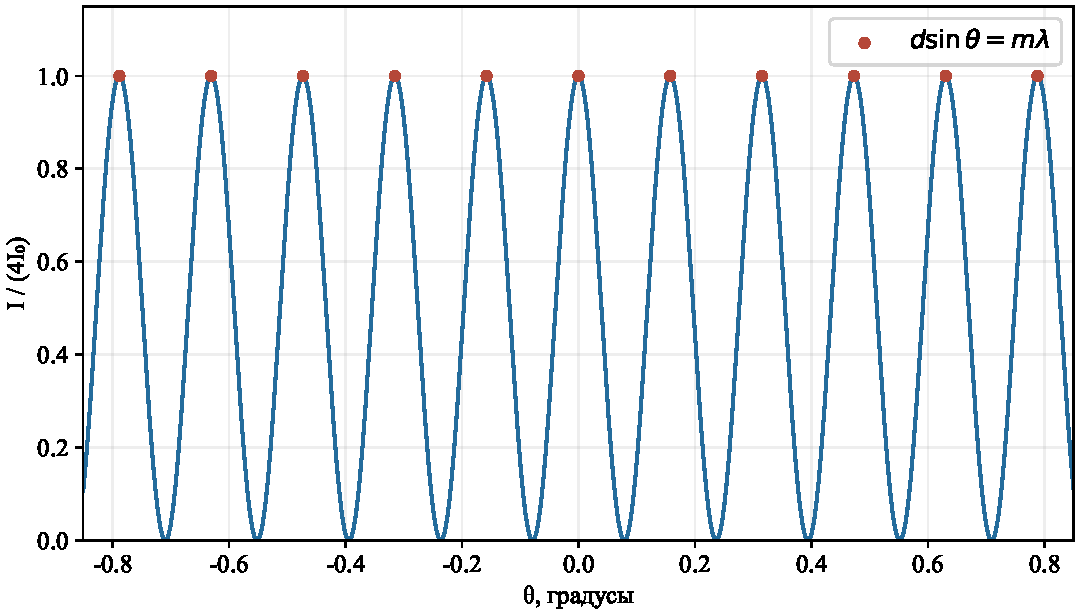
\includegraphics[width=0.93\textwidth]{task2_sources.pdf}
\caption{Угловая интерференционная картина. Точками отмечены максимумы
для порядков $m=-5,\ldots,5$.}
\end{figure}
Первый максимум расположен при $\theta_1=\SourceAngle{}^\circ$.
При малых углах $x\approx L\theta$, поэтому результат согласуется
с шириной полос из первого задания. В максимумах $I=4I_0$,
в минимумах $I=0$: складываются амплитуды полей, а интенсивность
пропорциональна квадрату амплитуды.

Свет в тёмной полосе не «уничтожается»: энергия перераспределяется
между направлениями наблюдения. Для устойчивой картины нужна
стабильная разность фаз за время регистрации. Два независимых бытовых
источника обычно такой картины не дают; в опыте Юнга два пучка получают
от одного источника. Применение --- интерферометры и контроль
формы оптических поверхностей.

\clearpage
\section{Интерференция в тонкой плёнке}
Принята система воздух--плёнка--воздух, толщина $t=2$ мкм.
Угол $\theta$ отсчитывается \emph{внутри} плёнки.
Для двух отражённых лучей разность фаз с учётом отражений:
\begin{equation}
 \Delta\varphi=\frac{4\pi nt\cos\theta}{\lambda}+\pi\pmod{2\pi},\qquad
 J(\theta)=\sin^2\frac{2\pi nt\cos\theta}{\lambda}.
\end{equation}
Здесь $J$ --- интенсивность, нормированная на максимум модели двух
равноамплитудных отражённых волн. Угловая зависимость коэффициентов
Френеля и многократные отражения не учитываются; $J$ не является
абсолютным коэффициентом отражения плёнки.
\begin{figure}[H]
\centering
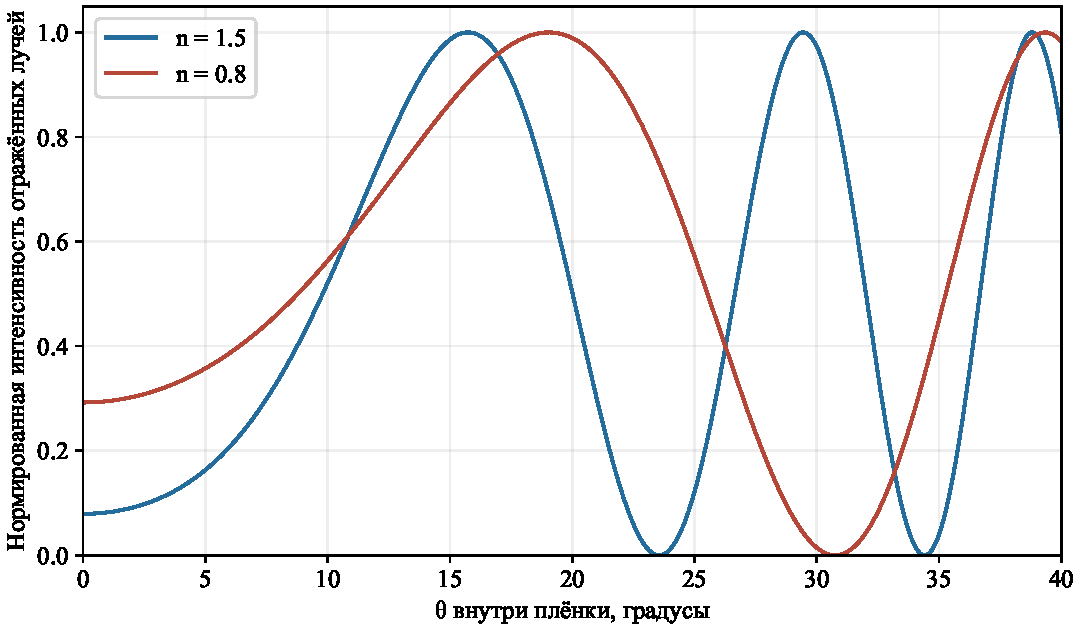
\includegraphics[width=0.9\textwidth]{task3_film.pdf}
\caption{Влияние показателя преломления на отражённую картину.}
\end{figure}
При одном относительном скачке фазы $\pi$ условия отражения:
\[
 \text{максимум: }2nt\cos\theta=(m+\tfrac12)\lambda,\qquad
 \text{минимум: }2nt\cos\theta=m\lambda.
\]
Для $n=1{,}5$ скачок возникает на верхней границе, для модельного
$n=0{,}8$ --- на нижней; относительный скачок остаётся равным $\pi$.
Поэтому изменение $n$ меняет оптическую толщину и положения экстремумов,
но само по себе не меняет местами правила максимумов и минимумов.
Случай $n=0{,}8$ --- модельный, он не описывает обычную мыльную плёнку.

Закон Снеллиуса: $\sin\alpha=n\sin\theta$, где $\alpha$ --- угол в воздухе.
Диапазон $0\le\theta\le40^\circ$ доступен обоим $n$;
при $n=1{,}5$ предельный внутренний угол $\arcsin(1/1{,}5)\approx41{,}81^\circ$.
Примеры --- цвета мыльных пузырей, измерение толщины покрытий,
просветляющие слои на линзах.

\clearpage
\section{Закон Малюса}
Амплитуда электрического поля после идеального анализатора равна
проекции поля на его ось: $E_{\mathrm{вых}}=E_0\cos\alpha$.
Поскольку $I\propto E^2$,
\begin{equation}
 \boxed{I(\alpha)=I_0\cos^2\alpha.}
\end{equation}
Здесь $I_0=1$ --- интенсивность уже линейно поляризованного света
\emph{перед анализатором}, $\alpha$ --- угол между его осью и поляризацией.
\begin{figure}[H]
\centering
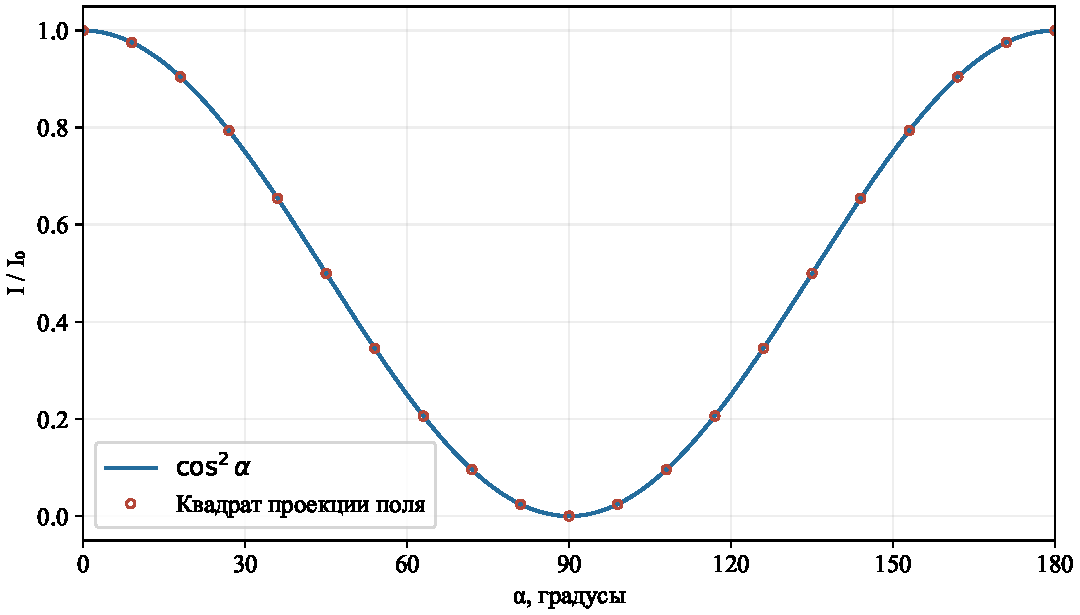
\includegraphics[width=0.92\textwidth]{task4_malus.pdf}
\caption{Закон Малюса и результат вычисления через проекцию поля.}
\end{figure}
Для углов $0^\circ$, $30^\circ$, $45^\circ$, $60^\circ$, $90^\circ$
получено $I/I_0=1$; 0,75; 0,50; 0,25; 0.
Расчёт проекции совпадает с законом Малюса с точностью округления.
При $90^\circ$ анализатор и поляризация скрещены; при $180^\circ$
интенсивность снова максимальна.

Если на первый идеальный поляризатор падает естественный свет,
он пропускает в среднем половину исходной интенсивности; затем
к этому поляризованному свету применяется закон Малюса.
Поляризаторы используются для ослабления бликов, регулирования
яркости и в жидкокристаллических дисплеях.

\clearpage
\section{Дифракция Фраунгофера}
Рассматривается дальняя зона либо эквивалентная фокальная плоскость линзы.
При малых углах $\sin\theta\approx x/L$. По умолчанию $L=2$ м,
а $I_0=1$ --- центральная интенсивность соответствующей картины.

\subsection{Одиночная щель}
\begin{equation}
 \frac I{I_0}=\left(\frac{\sin\beta}{\beta}\right)^2,\qquad
 \beta=\frac{\pi ax}{\lambda L},\qquad
 x_m=\frac{m\lambda L}{a},\quad m=\pm1,\pm2,\ldots
\end{equation}
\begin{figure}[H]
\centering
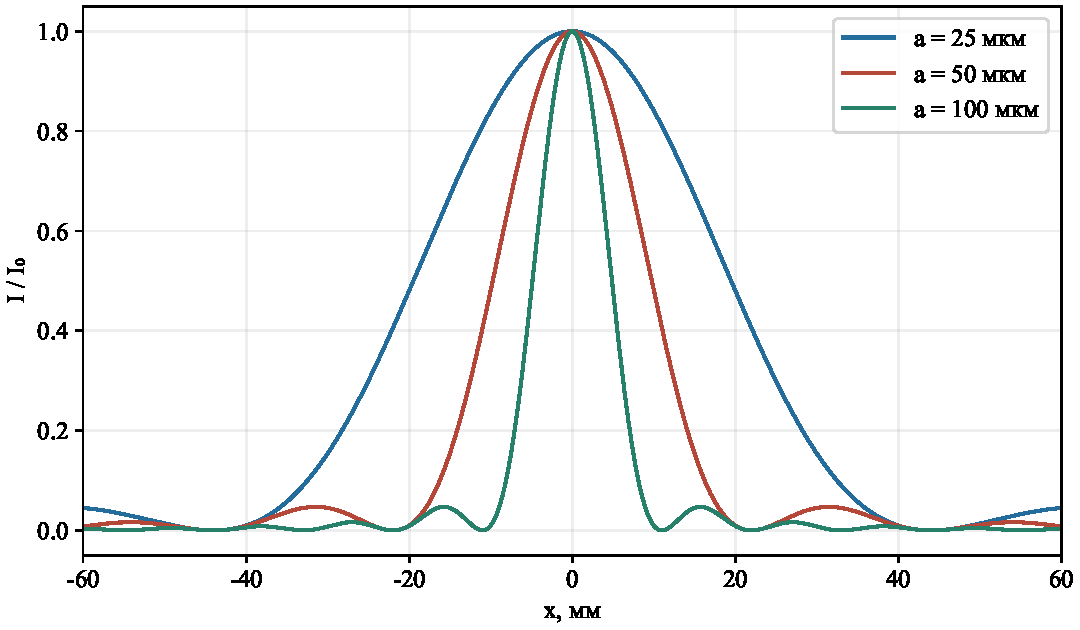
\includegraphics[width=0.92\textwidth]{task5a_single_slit.pdf}
\caption{Дифракция на щели при трёх значениях ширины $a$.}
\end{figure}
При $a=50$ мкм первые нули $x=\pm\SingleZero$ мм,
ширина центрального максимума $2\lambda L/a=\SingleWidth$ мм.
Он вдвое шире интервала между соседними минимумами с одной стороны.
Уменьшение щели расширяет угловое распределение: характерный масштаб
$\theta\sim\lambda/a$. Выбранные $a=25$--$100$ мкм намного больше
$\lambda=0{,}55$ мкм, но дают хорошо различимую картину на метровом расстоянии.

В центре $\lim_{\beta\to0}\sin\beta/\beta=1$, поэтому интенсивность
конечна. В программе используется функция
$\operatorname{sinc}(u)=\sin(\pi u)/(\pi u)$ с аргументом $\beta/\pi$.
Применение --- определение размеров щелей и оценка
дифракционного расширения лазерного пучка.

\clearpage
\subsection{Круглое отверстие: пятно Эйри}
Выбран радиус отверстия $R=0{,}10$ мм, диаметр $D_{\mathrm{отв}}=2R=0{,}20$ мм:
\begin{equation}
 \frac{I(r)}{I_0}=\left[\frac{2J_1(z)}z\right]^2,\qquad
 z=\frac{2\pi Rr}{\lambda L}.
\end{equation}
\begin{figure}[H]
\centering
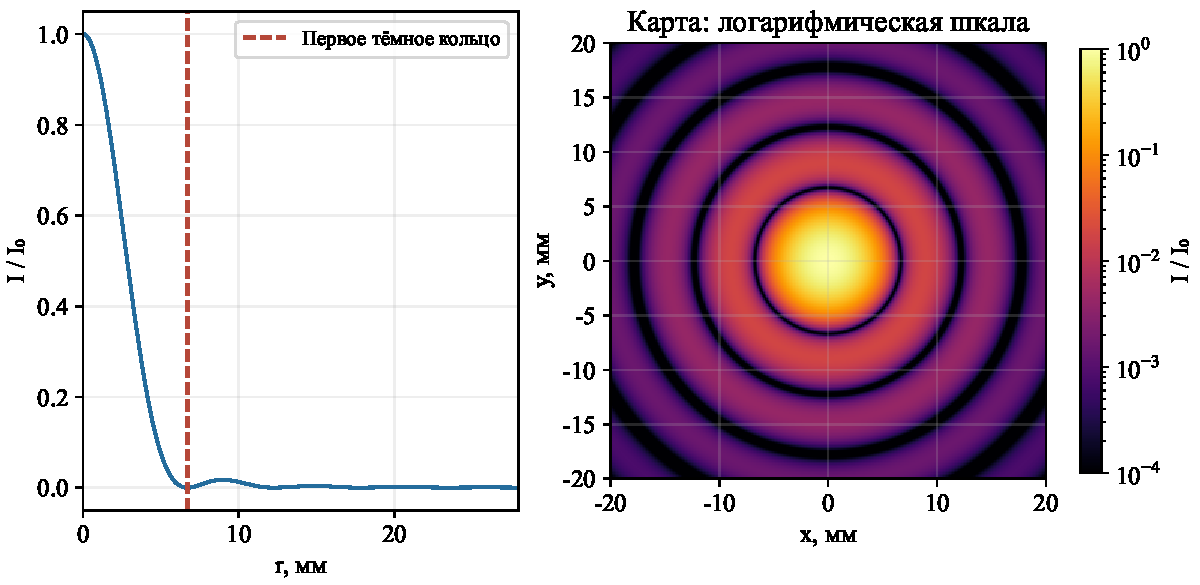
\includegraphics[width=0.99\textwidth]{task5b_airy.pdf}
\caption{Радиальный профиль и двумерная картина Эйри. Логарифмическая
цветовая шкала справа позволяет увидеть слабые кольца.}
\end{figure}
Первый положительный нуль $J_1$ равен $z_1\approx3{,}831706$:
\begin{equation}
 r_1=\frac{z_1\lambda L}{2\pi R}=\AiryRadius\ \text{мм}
 \approx0{,}61\frac{\lambda L}{R}
 =1{,}22\frac{\lambda L}{D_{\mathrm{отв}}}.
\end{equation}
Это радиус до первого тёмного кольца. Коэффициент $1{,}22$
используется с \emph{диаметром}, а $0{,}61$ --- с радиусом отверстия.
В центре предел $2J_1(z)/z=1$ обрабатывается отдельно.

Точечный объект изображается пятном конечного размера.
По критерию Рэлея два некогерентных точечных объекта различимы, когда
центр одного пятна приходится на первый минимум другого:
$\theta_{\mathrm R}\approx1{,}22\lambda/D_{\mathrm{отв}}$.
Увеличение диаметра уменьшает пятно и улучшает разрешение
телескопа, микроскопа или камеры.

\clearpage
\subsection{Две щели: интерференция под дифракционной огибающей}
Ширина каждой щели $a=50$ мкм; сравниваются $d=0{,}20$ и $0{,}40$ мм:
\begin{equation}
 \frac I{I_0}=\left(\frac{\sin\beta}{\beta}\right)^2\cos^2\delta,
 \qquad\beta=\frac{\pi ax}{\lambda L},\quad
 \delta=\frac{\pi dx}{\lambda L}.
\end{equation}
\begin{figure}[H]
\centering
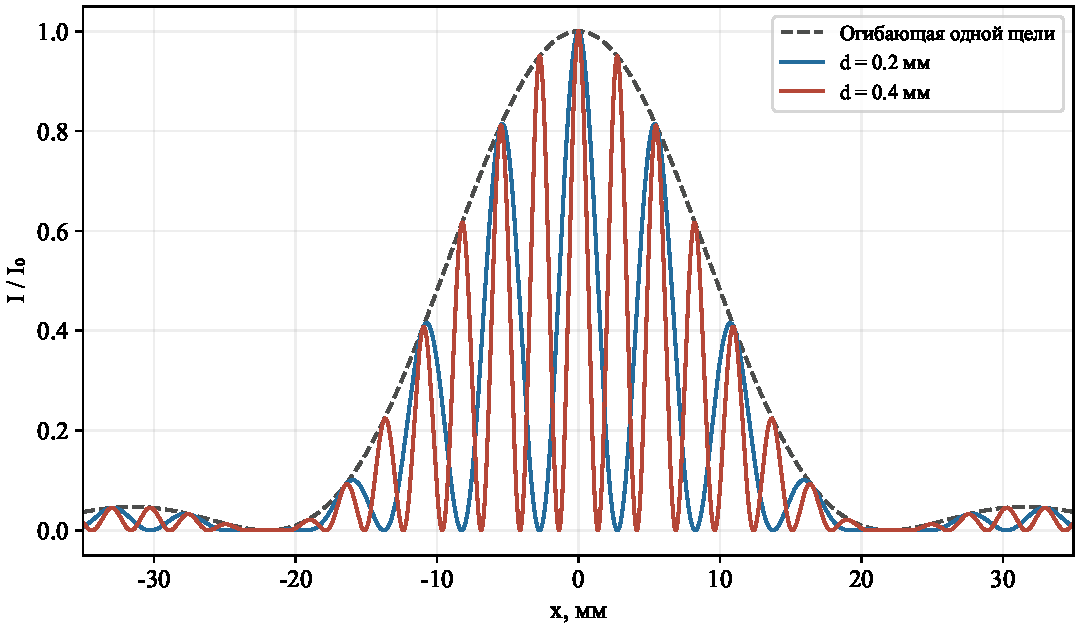
\includegraphics[width=0.94\textwidth]{task5c_double_slit.pdf}
\caption{Узкие интерференционные полосы внутри огибающей одиночной щели.}
\end{figure}
Параметр $a$ определяет широкую дифракционную огибающую,
а $d$ --- шаг узких полос. При удвоении $d$ шаг уменьшается
с 5,5 до 2,75 мм, огибающая сохраняется. Если интерференционный максимум
попадает на дифракционный минимум, соответствующий порядок гасится.
Здесь $d/a=4$ или 8, поэтому, в частности, порядок $m=4$ или $m=8$
совпадает с первым нулём огибающей.

В отличие от идеальных точечных источников, щели имеют конечную ширину:
излучение разных участков каждой щели также интерферирует.
Опыт Юнга показывает волновую природу света и позволяет определить
длину волны по расстоянию между полосами.

\clearpage
\subsection{Многощелевая решётка}
Период решётки $d_g=10$ мкм; сравниваются $N=5$, 10 и 20 узких щелей.
Их собственная дифракционная огибающая в модели не учитывается:
\begin{equation}
 \frac{I(\theta)}{I(0)}=
 \frac1{N^2}\left[\frac{\sin(N\beta_g)}{\sin\beta_g}\right]^2,
 \qquad\beta_g=\frac{\pi d_g\sin\theta}{\lambda}.
\end{equation}
\begin{figure}[H]
\centering
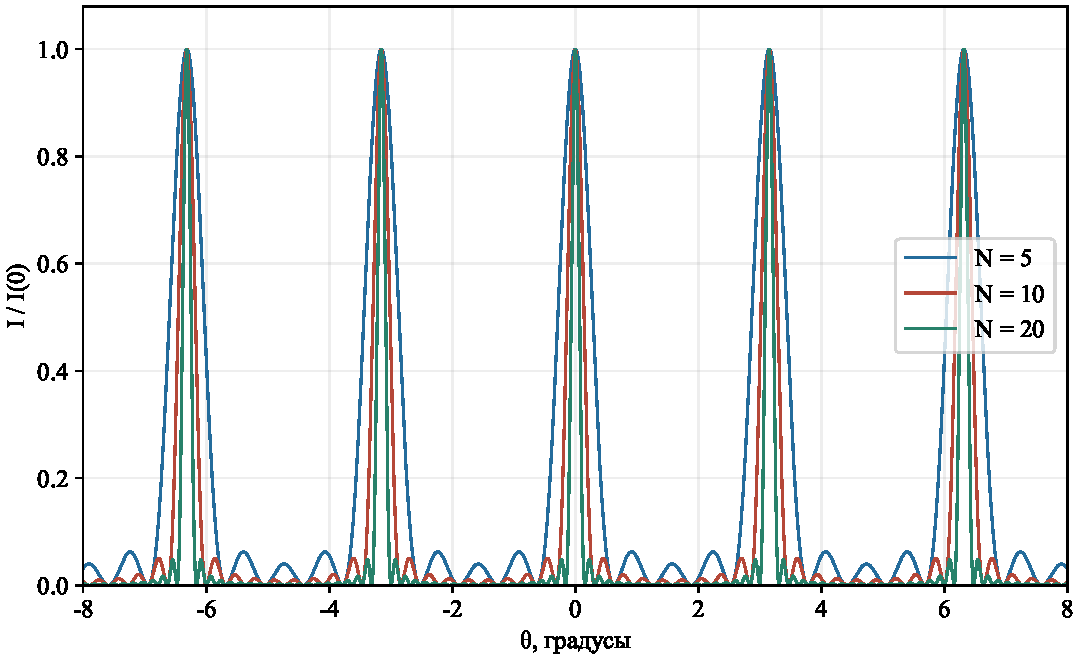
\includegraphics[width=0.92\textwidth]{task5d_grating.pdf}
\caption{Нормированные картины решёток с разным числом щелей.}
\end{figure}
Главные максимумы удовлетворяют $d_g\sin\theta_m=m\lambda$;
первый находится при $\theta_1=\GratingAngle{}^\circ$.
Множитель $1/N^2$ обеспечивает $I(0)=1$; без нормировки пиковая
интенсивность при одинаковом освещении каждой щели растёт как $N^2$.
В программе складываются комплексные поля щелей, поэтому
устранимая неопределённость в главных максимумах не возникает.

Ширина центрального главного максимума между первыми нулями
$2\arcsin[\lambda/(Nd_g)]$ уменьшается примерно как $1/N$.
Разные длины волн дают разные углы максимумов: решётка разделяет
свет на спектр, а большее число освещённых штрихов помогает различать
близкие спектральные линии.

\section*{Вывод}
Интерференция перераспределяет энергию, поляризатор выбирает проекцию
поля, дифракция определяет расширение пучка и предел разрешения.
Полученные зависимости объясняют работу интерферометров, оптических
покрытий, поляризационных фильтров и спектральных приборов.
\end{document}
